\documentclass{article}
\usepackage{float}
\usepackage{natbib}
\title{Verification Package: examples using weather forecasts.}
\author{Matthew Pocernich}


%% \usepackage{a4wide}

% \VignetteIndexEntry{An example of verifying weather forecasts.}
% \VignetteDepends{fields, boot, CircStats}
% \VignetteKeyword{weather}

\setlength{\textwidth}{6.5in} \setlength{\textheight}{9in}
%\setlength{\oddsidemargin}{-0.5in}
%\setlength{\evensidemargin}{-0.5in}
\setlength{\oddsidemargin}{0in}
\setlength{\evensidemargin}{0in}
\setlength{\topmargin}{-0.75in}
% \renewcommand{\baselinestretch}{1.5}
\newcommand{\ee}{\end{equation}} 
\newcommand{\be}{\begin{equation}} 
\newcommand{\ec}{\end{center}} 
\newcommand{\bc}{\begin{center}} 
\newcommand{\eea}{\end{eqnarray}} 
\newcommand{\bea}{\begin{eqnarray}} 
%\newcommand{\sumprime}{\mathop{{\sum}'}} 
\newcommand{\bd}{\begin{description}} 
\newcommand{\ed}{\end{description}} 
\newcommand{\bi}{\begin{itemize}} 
\newcommand{\ei}{\end{itemize}} 
\newcommand{\pa}{\partial} 
\newcommand{\hor}{\left(\frac{h}{R_0}\right)} 
 

\usepackage{c:/PROGRA~1/r/R-27~1.0DE/share/texmf/Sweave}
\begin{document}

\maketitle
The National Center for Atmospheric Sciences (NCAR) develops and
implements weather and climate models.
Verification statistics play a key role in this cycle.
Functions in the \textbf{verification} library contains functions that 
have been developed in this process. 

While the examples in this library focus on atmospheric topics,
they are written to be applicable to any situations in which there is
a prediction or forecast and an observation of the outcome.  The
statistics used to verify and study weather and climate forecasts are
shared by many fields.  Most notably, these include the fields of
medicine (where the name misclassification statistics is favored) and
signal detection theory.  Some useful references are listed below.   

The type of predictions and observations determine which methods 
are appropriate for verification. The following types of predictions are currently supported:
binary, categorical, continuous, probabilistic and distributions.  
The presence or absence of fog is an example of binary data. A
forecast for turbulence expressed in terms of low, moderate and
extreme is a categorical forecast. The
chance of precipitation is an example of a probabilistic forecast.  A
temperature forecast as a single value is (essentially) a continuous variable.
People are finding it increasingly useful to express
the uncertainly of a point forecast.  In this case, the forecast may
be expressed as a distribution. 

\section{Finley's Tornado}

Any discussion of verification must begin in the beginning and for
weather, that means John Finley and tornado forecasts.  In 1884, John
Finley using the telegraph, created yes/no tornado forecasts for 18
regions of the US \cite{finley84}.  Citing the results in Table
\ref{fin}, he explained that his method was 96.6 accurate.
     
\begin{table}[H]
\begin{center}
 \caption{\label{fin}Finley Tornado Data  }
\begin{tabular}{|c||c|c|} \hline 
&  \multicolumn{2}{c}{Forecasts}\\ \hline
Observation& Yes & No \\ \hline
Yes & 28 &72  \\
No &  23 & 2680 \\ \hline
\end{tabular}
\end{center}
\end{table}  


\begin{Schunk}
\begin{Soutput}
fields is loaded use help(fields) for an overview of this library  
  Some name changes have been made to several common functions: 
  exp.-> Exp. and rad. -> Rad. See help( Exp.cov)
\end{Soutput}
\begin{Soutput}
[1] " Assume data entered as c(n11, n01, n10, n00) Obs*Forecast"
\end{Soutput}
\begin{Soutput}
The forecasts are binary, the observations are binary.
The contingency table for the forecast 
     [,1] [,2]
[1,]   28   72
[2,]   23 2680

PODy =  0.549 
TS   =  0.2276 
ETS  =  0.216 
FAR  =   0.72 
HSS  =  0.3553 
PC   =  0.9661 
BIAS =  1.961 
\end{Soutput}
\end{Schunk}

It was quickly pointed out that since tornados are so rare, if one
always forecasted no tornado, the percent correct would be  98.2% of
the time.  The downside to this that the probability of detecting a
tornado (PODy) drops to 0.

\begin{Schunk}
\begin{Soutput}
[1] " Assume data entered as c(n11, n01, n10, n00) Obs*Forecast"
\end{Soutput}
\begin{Soutput}
The forecasts are binary, the observations are binary.
The contingency table for the forecast 
     [,1] [,2]
[1,]    0    0
[2,]   51 2752

PODy =      0 
TS   =      0 
ETS  =      0 
FAR  =    NaN 
HSS  =      0 
PC   =  0.9818 
BIAS =      0 
\end{Soutput}
\end{Schunk}

Note: \textbf{verify} is an overloaded function
whose behavior is dictated by the types of forecasts and
observations.  By default, \textbf{verify} assumes that the forecast is
probabilistic and the observation is binary.  In the preceding
example, since both the forecast and observation are binary, the
forecast type needs to be described.
  
\section{Verifying a precipitation forecast} 

While variables such as temperature, humidity and wind speed
are traditionally forecast as a point forecast, precipitation
has historically been forecast as a probability.  The following
example use precipitation forecast made by the Finnish Meteorological
Institute \cite{fin}.  This data is included as a sample data set in
the verification package.

\begin{Schunk}
\begin{Soutput}
If baseline is not included, baseline values  will be calculated from the  sample obs. 
\end{Soutput}
\begin{Soutput}
The forecasts are probabilistic, the observations are binary.
Sample baseline calculated from observations.
Brier Score (BS)           =  0.1445 
Brier Score - Baseline     =  0.1793 
Skill Score                =  0.1942 
Reliability                =  0.02536 
Resolution                 =  0.06017 
Uncertainty              =  0.1793 
\end{Soutput}
\end{Schunk}

Typically, the probability of rain is expressed as one of a finite
number of probabilities such as 10\%, 20\%, etc.  Its not typical to 
see a forecast saying there is a 34.7\% chance of rain.  For automated
forecasts  or one's which aren't rounded a continuous range
of values between 0 and 1 are possible.   The \textit{bins} option addresses this
distinction.  If bins = TRUE,  forecast are placed into bins and
assigned the center values.  By default these bins are described by
the \textit{threshold} parameter and are (0, 0.1, ..., 0.9, 1).  If
FALSE, as in the case for precipitation forecasts, each forecast is
considered individually.  This becomes important when calculating
statistics such as the Brier statistic.

\begin {center}
\begin{figure}[H]
\begin{Schunk}
\begin{Sinput}
> plot(A)
\end{Sinput}
\end{Schunk}
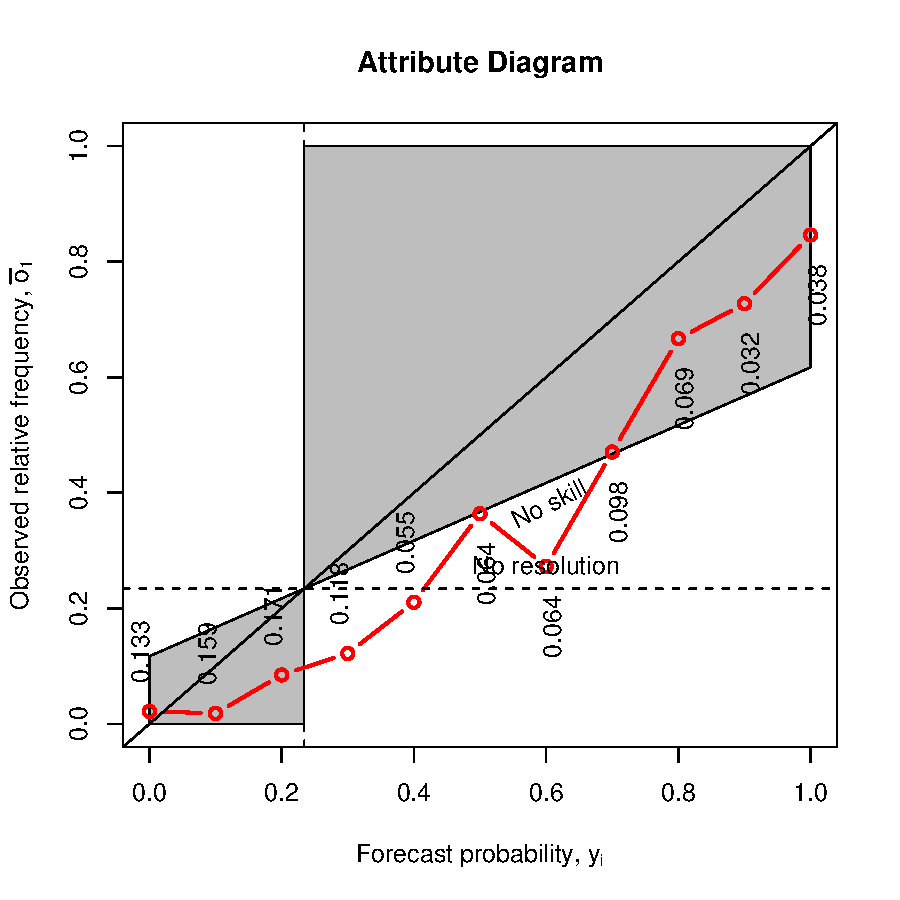
\includegraphics{verification-004}
\caption{\label{att.diag} Attribute Diagram for light precipitation forecast}
\end{figure}
\end{center}    

While the  attribute diagram (Figure \ref{att.diag} ) is the default diagram
for a probabilistic forecast, there are other very useful diagrams.
The receiver operating characteristics (ROC) plot is also commonly
used.  A ROC plot displays the relation between false alarms and hits
(successfully forecasted events) across a range of thresholds. Figure
\ref{roc1}  shows a ROC plot for the probability of precipitation
forecast.  Since one wants a high ratio of hits to false alarms, the
better the forecast, the further into the upper left hand corner the
plot extends.  This plot displays two lines.  The black, un-smooth
line is the empirical ROC plot.  At each threshold, points are
plotted.  The smoother line is the result of fitted a binormal
distribution to the points.  For a perfect forecast, the area under
the ROC curve would equal 1.  In this example, the area under the
curve is shown in the legend box.  First the area under empirical
curve is shown followed by the area under the bi-normal curve. 

\begin {center}
\begin{figure}[H]
\begin{Schunk}
\begin{Sinput}
> mod24 <- verify(d$obs_norain, d$p24_norain, bins = FALSE)
\end{Sinput}
\begin{Soutput}
If baseline is not included, baseline values  will be calculated from the  sample obs. 
\end{Soutput}
\begin{Sinput}
> mod48 <- verify(d$obs_norain, d$p48_norain, bins = FALSE)
\end{Sinput}
\begin{Soutput}
If baseline is not included, baseline values  will be calculated from the  sample obs. 
\end{Soutput}
\begin{Sinput}
> roc.plot(mod24, plot.thres = NULL)
> lines.roc(mod48, col = 2, lwd = 2)
> leg.txt <- c("24 hour forecast", "48 hour forecast")
> legend(0.6, 0.4, leg.txt, col = c(1, 2), lwd = 2)
\end{Sinput}
\end{Schunk}
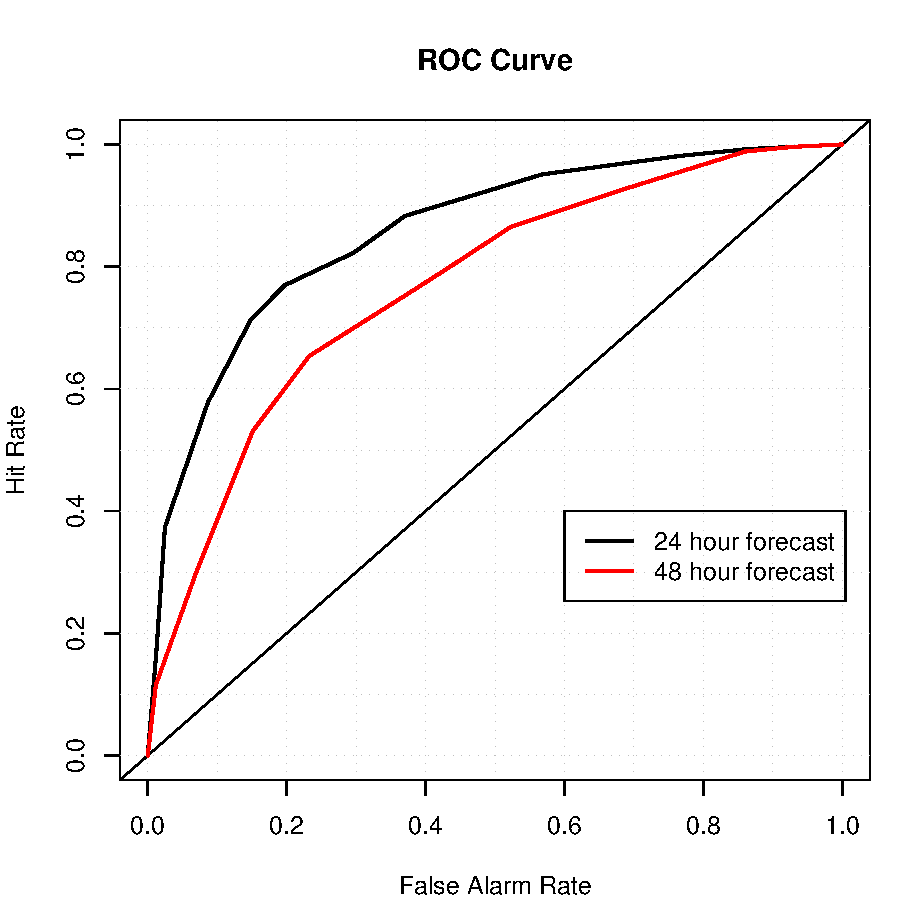
\includegraphics{verification-005}
\caption{\label{roc1} Receiver operating characteristic curve for chance of 
rain forecast at 24 and 48 hour lead times.}
\end{figure}
\end{center}    

Unfortunately, estimating and expressing the uncertainty in these
curves  is seldom done.  The verification packages offers a couple
options for this.  The data can be bootstrapped, to estimate the
variance at the set thresholds (Figure \ref{roc2}).   

\begin {center}
\begin{figure}[H]
\begin{Schunk}
\begin{Sinput}
> B <- roc.plot(A, CI = TRUE, n.boot = 100)
\end{Sinput}
\end{Schunk}
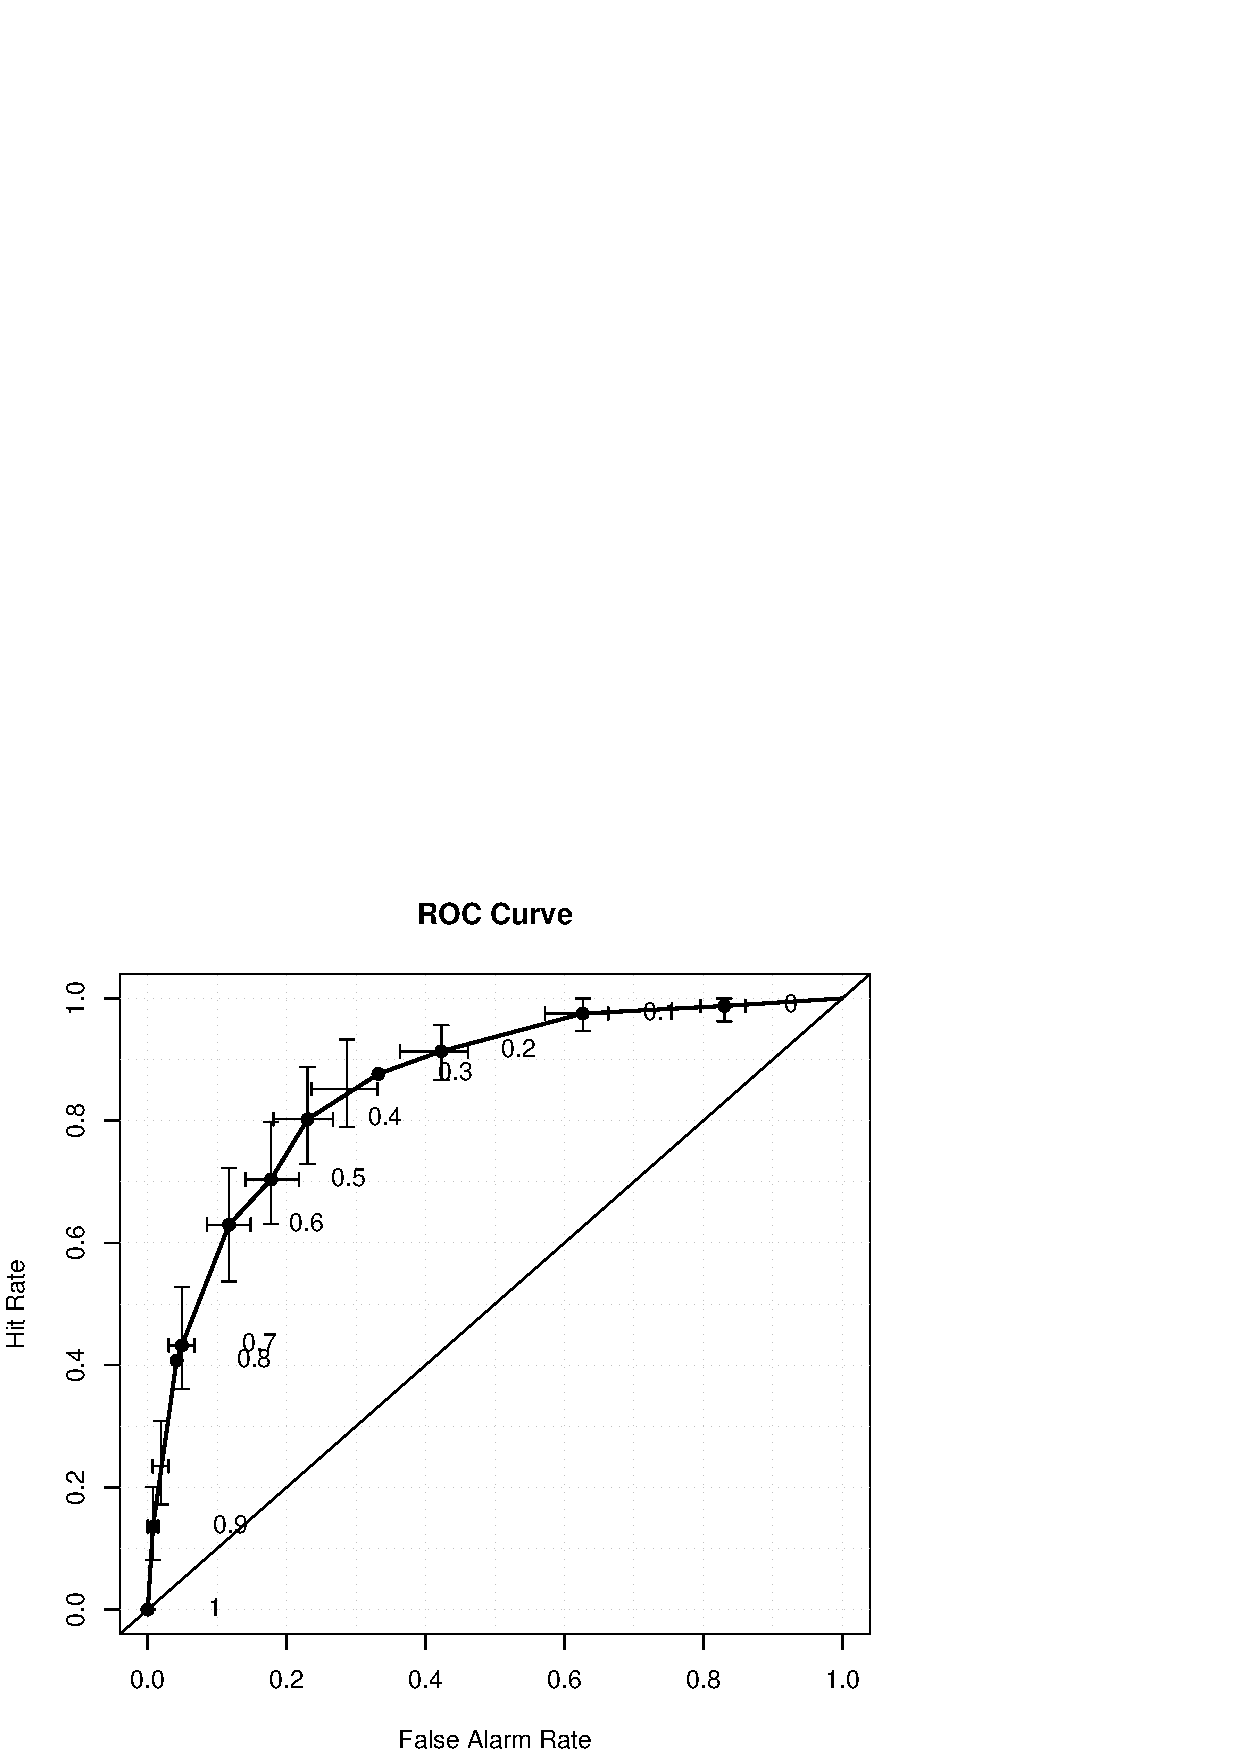
\includegraphics{verification-006}
\caption{\label{roc2} ROC curve with bootstrapped confidence
intervals. }
\end{figure}
\end{center}    

\section{Value Diagrams}

The utility of a forecast varies based upon the needs and concerns of
an individual user.  Value diagrams can be used to determine over what
range of cost-lost (cl) ratios a forecast will provide value.  The cost-lost
ratio is the ratio of the cost of preparing for an event that doesn't
occur over the losses that will occur if one is not prepared.  Small
values indicate that the costs to prepare are small in relation to the
losses.  The peaks of this graph occurs at the baseline average of an
event.  Figure \ref{val1} is an illustration of a value diagram for
the Finnish precipitation data.

\begin {center}
\begin{figure}[H]
\begin{Schunk}
\begin{Sinput}
> value(d$obs_rain, d$p24_rain, main = "Rain-No Rain Forecast", 
+     cl = seq(0.01, 0.99, 0.05), all = TRUE)
\end{Sinput}
\end{Schunk}
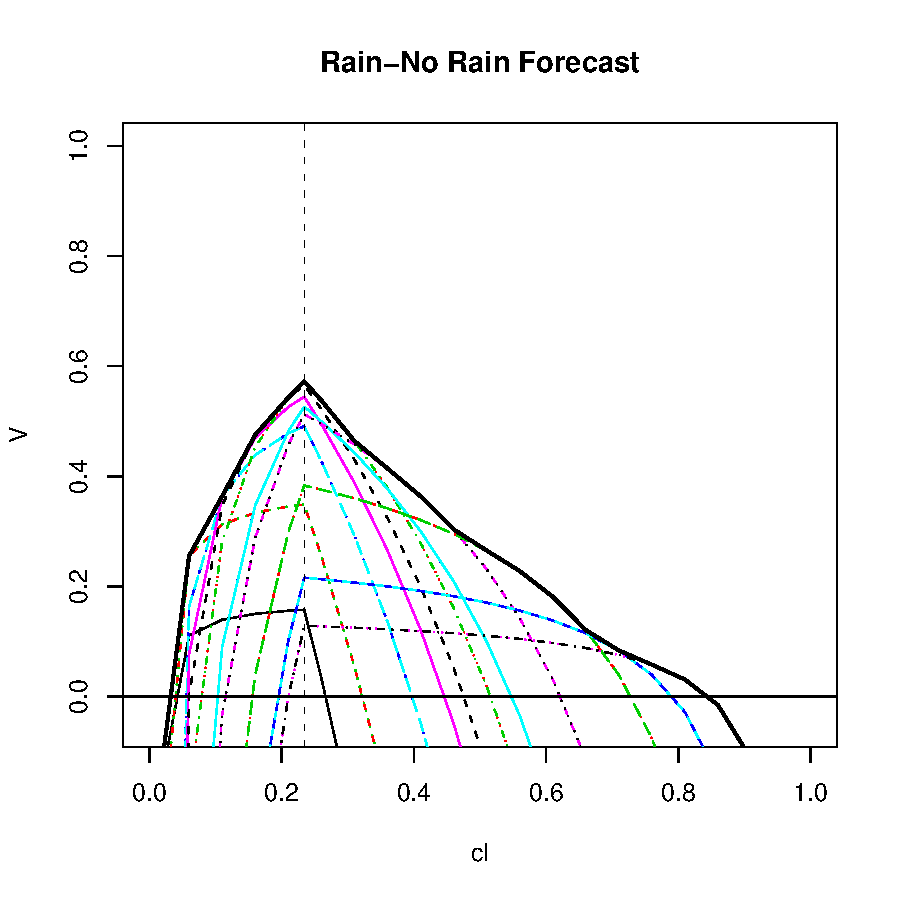
\includegraphics{verification-007}
\caption{\label{val1} Value diagram of light precipitation forecast. }
\end{figure}
\end{center}    

  

\section{Discrimination Plot}
A discrimination plot illustrates the the distributions of forecasts
grouped by different types of distributions.  Ideally, one would see a
distinct histograms (Figure \ref{disc1}) .  

\begin {center}
\begin{figure}[H]
\begin{Schunk}
\begin{Sinput}
> discrimination.plot(disc.dat$group.id, disc.dat$frcst, main = "Sample Plot")
\end{Sinput}
\end{Schunk}
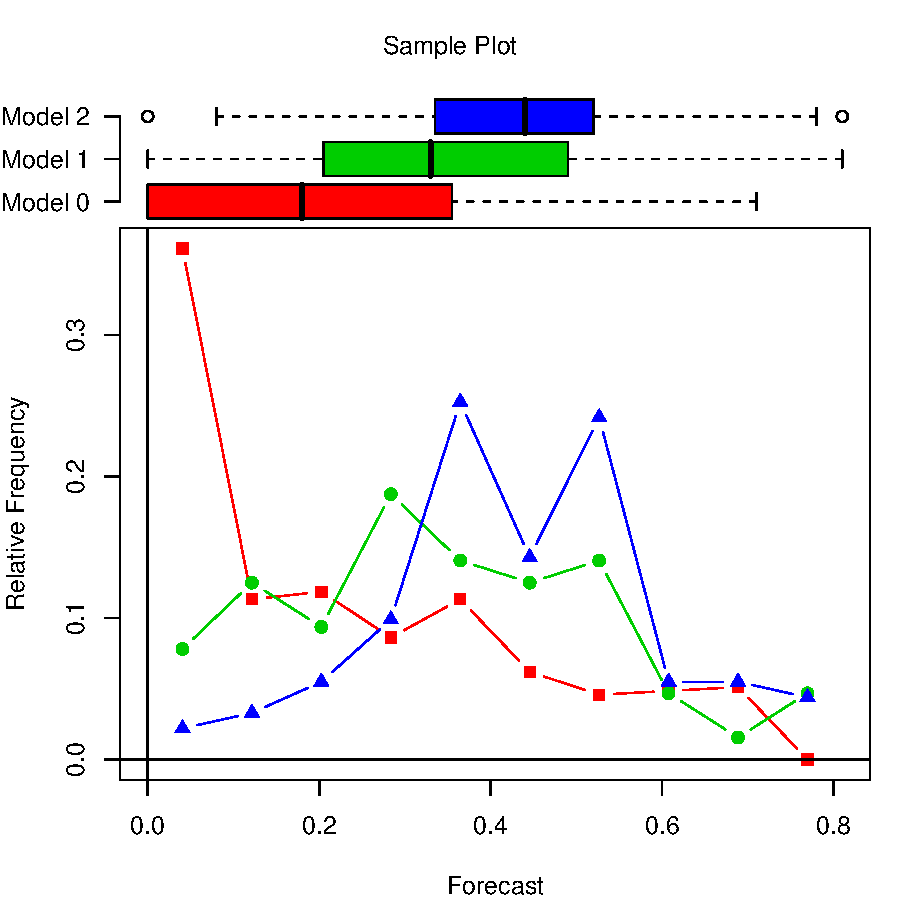
\includegraphics{verification-008}
\caption{\label{disc1} Discrimination plot using aviation forecast. }
\end{figure}
\end{center}    

\section{Reliability Diagram}
Related to the attribute diagram is the reliability diagram. A
reliability diagram can be used to compare multiple forecasts.  Figure
\ref{rel1} is an example using data from \cite{wilks95}.

\begin {center}
\begin{figure}[H]
\begin{Schunk}
\begin{Sinput}
> y.i <- c(0, 0.05, seq(0.1, 1, 0.1))
> obar.i <- c(0.006, 0.019, 0.059, 0.15, 0.277, 0.377, 0.511, 0.587, 
+     0.723, 0.779, 0.934, 0.933)
> prob.y <- c(0.4112, 0.0671, 0.1833, 0.0986, 0.0616, 0.0366, 0.0303, 
+     0.0275, 0.245, 0.022, 0.017, 0.203)
> obar <- 0.162
> reliability.plot(y.i, obar.i, prob.y, titl = " Wilks Data", legend.names = c("Model A"))
\end{Sinput}
\end{Schunk}
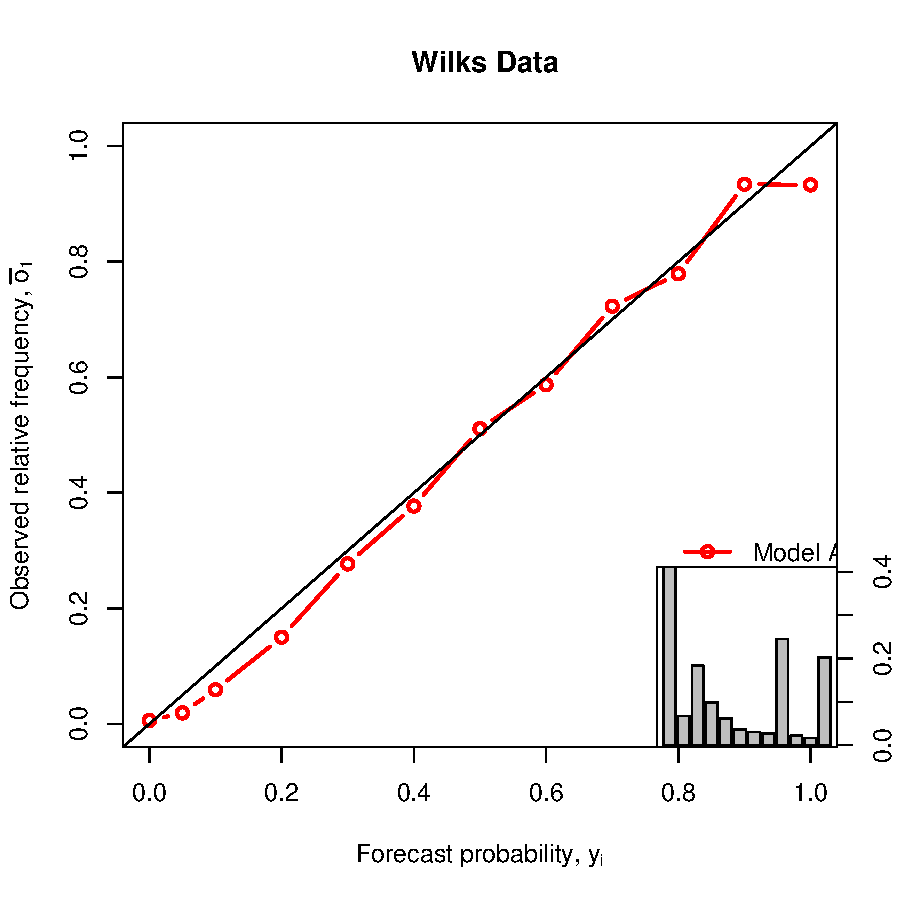
\includegraphics{verification-009}
\caption{\label{rel1} Reliability diagram of Wilks example. }
\end{figure}
\end{center}    


\nocite{*}
\bibliographystyle{ametsoc_fussy_tmp}
%\bibliographystyle{plain}
\bibliography{guide}

\end{document}
